\section{Nombre: Mictlecayotl}  \label{per:mictlecayotl}

\subsection{Descripción:}
Mictlecayotl es una deidad guerrera por lo que su vestimenta está orientada a la batalla, porta una armadura ligera que le permite realizar rápidos ataques de viento, pero el costo de su rapidez es la poca defensa ante poderosos ataque que ofrece la armadura. En los antebrazos usa unos protectores que por su diseño también le permiten desgarrar a sus enemigos si estos se encuentran cerca de ella. Sus codos y sus rodillas son protegidas por unas conchas recogidas de los lagos del octavo nivel del Mictlán, estas conchas poseen la habilidad de proteger contra encantamientos que alteran el pensamiento a quien los porta. Lleva el cabello recogido en una coleta para evitar que le estorbe en combate. Su rostro esta maquillado con pintura para guerra. A manera de recordatorio de su antigua posición en la jerarquía divina porta un collar y aretes de oro. Es una mujer de estatura mediana, espalda ancha y piernas fuertes. 
\\
\par
Mictlecayotl se caracteriza por ser de actitud paciente y callada pero orgullosa. No tiene problemas para relacionarse con otros dioses. Es una persona reservada que difícilmente hablara sobre ella y sus problemas, pero está dispuesta a escuchar a los demás y a ayudarlos. Siente una gran compasión por la raza humana por lo que trata de que los difuntos encuentren la paz en su paso por su nivel del infierno por lo que no es extraño verla ayudando a quienes demuestren ser dignos.  
\\
\par
\textbf{Nota de diseño}: Su paleta de colores será una variación de diferentes tonalidades de azul. 	  
\subsection{Status:}
	\begin{itemize}
		\item Personaje no jugable.
		\item Enemigo jefe.
	\end{itemize}
\subsection{Imagen}
	Ver figura \ref{fig:MictlecayotlDiseno}
	\begin{figure}
					\centering
					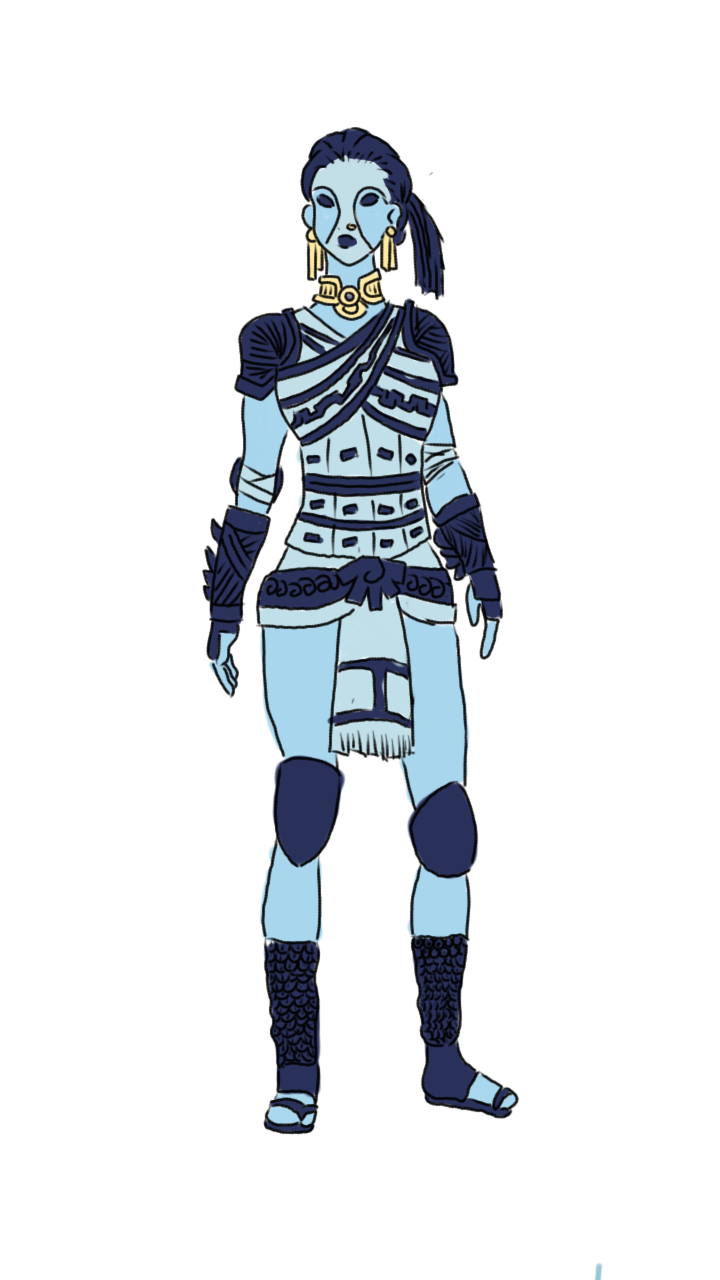
\includegraphics[height=0.3 \textheight]{Imagenes/vientoNorte}
					\caption{Concepto de diseño de Mictlecayotl.}
					\label{fig:MictlecayotlDiseno}
	\end{figure}
\subsection{Concepto:}
\begin{itemize}
	\item \textbf{Historia antes del juego:}
	Mictlecayotl es la diosa del viento del norte y esposa del dios del viento Ehécatl. Durante la época anterior al exilio de Quetzalcóatl, Mictlecayotl vivía junto a su esposo en uno de los trece cielos. Luego de que su esposo se enamorara de una humana,  Mictlecayotl decide observar a los humanos para comprender que es lo que tienen de especiales, acción que la llevaría a comprender que lo que hacía bella la existencia humana era lo efímera y frágil que ésta podía ser, siendo estas características lo que impulsaba a las personas a hacer cosas extraordinarias al buscar la inmortalidad en el recuerdo popular. Observar a los humanos le permitiría además formar una amistad con Quetzalcóatl.
	\\
	\par
	Cuando Quetzalcóatl se exilia luego de la caída de Tula,  Mictlecayotl se muestra deprimida. El exilio de Quetzalcóatl trae consigo una serie de cambios en los trece cielos. De un momento a otro todos los dioses que habían simpatizado con Quetzalcóatl se ven degradados de rango y en su lugar eran puestos los simpatizantes de Tezcatlipoca. Mictlecayotl logra mantener su posición jerárquica a pesar de su amistad con Quetzalcóatl. Y al cabo de unos meses regresa a sus tareas como protectora del viento del norte. Sin embargo, una vez que descubre la verdad tras el exilio de Quetzalcóatl,  Mictlecayotl trata de asesinar a Tezcatlipoca sin éxito. Ehécatl logra convencer al dios negro de que no asesine a Mictlecayotl. Tezcatlipoca le perdona la vida a la diosa, pero determina que ella debe de sufrir un castigo por su crimen. Es así como Mictlecayotl es separada de Ehécatl y es enviada al Mictlán para fungir como guardiana del cuarto nivel del Mictlán, permitiéndole ver a Ehécatl únicamente cuando los vientos helados del norte salieran del Mictlán hacia la tierra de los mortales durante los inviernos.			
	\item \textbf{Historia durante el juego:}
	Como guardiana del cuarto nivel del Inframundo, Mictlecayotl tiene la obligación de frenar a Xolotl en su cruzada por el Mictlán. Luego de la caída de Xochitonal, Mictlantecutli ordenara a los guardianes del Mictlan proteger el inframundo y evitar a toda costa el avance de Xolotl. Mictlecayotl encontrará la muerte en su enfrentamiento con Xolotl y Malinalli pero antes de desaparecer Xolotl le contará que durante su exilio tuvo la oportunidad de encontrarse a Quetzalcóatl.
	\item \textbf{Relaciones:}
	\begin{itemize}
		\item \textbf{Xolotl:} Considerado como un traidor. La opinión de Mictlecayotl cambia cuando Xolotl le cuenta que trato de detener a Tezcatlipoca la noche que éste provoco el exilio de Quetzalcóatl. Mictlecayotl le agradece a Xolotl por tratar de ayudar a Quetzalcóatl y le pide que se encargue de Tezcatlipoca (ver aparatado \ref{per:xolotl}).
		
		\item \textbf{Ehécatl:} Esposo de Mictlecayotl. Ambos comparten una relación de respeto y apoyo mutuo. 
		
		\item \textbf{Quetzalcóatl:} Amigo de Mictlecayotl. Es el dios al que más admira y al único al que reconoce como digno de ser el líder de los trece cielos. Mictlecayotl espera su regreso para que traiga fin al nuevo orden que Tezcatlipoca ha instaurado (ver aparatado \ref{per:quetzalcoatl}).
		
		\item \textbf{Tezcatlipoca:} Enemigo de Mictlecayotl. Trató de matarlo en una ocasión (ver aparatado \ref{per:tezcatlipoca}.  
	\end{itemize}			  
\end{itemize}


\subsection{Encuentro:}
\begin{itemize}
	\item Su primera aparición es en la cinemática 9 (ver aparatado \ref{Cin:Cinematica09}). 
	\item Su primer y único encuentro con Malinalli es en el quinto nivel del juego (ver aparatado \ref{Nivel:Niv05}).
\end{itemize}
\subsection{Habilidades:}
Como diosa del viento, la principal habilidad de Mictlecayotl es manipular el viento con el que crea diferentes ataques como:
\begin{itemize}
	\item Tornado (ver aparatado \ref{hab.tornado}).
	\item Ventisca (ver aparatado \ref{ventisca}).
\end{itemize}

Sus habilidades de viento también le permiten desvanecerse en el aire y aparecer en una posición ventajosa para su ataque.
\subsection{Armas:}
Trepa viento (ver aparatado \ref{Arma:EspadaMictlecayotl}).
\subsection{Ítems:}
Sin ítems.
\subsection{Bloques de animación}
	\begin{itemize}
		\item Animación disparar viento.
		\item Animación invocar tornado.
		\item Animación volar.
		\item Animación recibir daño.
		\item Animación morir.
	\end{itemize} 